\documentclass{article}
\usepackage{mathbbol}
\usepackage{graphicx}
% \usepackage{multirow}
% \usepackage{amsmath}

\graphicspath{ {./images/} }
\renewcommand{\arraystretch}{2.5}
\newcommand{\definition}[1]{\paragraph*{\underline{Definition}: #1}}
\newcommand{\property}[1]{\paragraph*{\underline{Property}: #1}}
\renewcommand{\vec}[1]{\overrightarrow{#1}}
\newcommand{\scmul}[2]{\vec{#1} \cdot \vec{#2}}
\newcommand{\twodivec}[3]{\vec{#1} \begin{pmatrix}#2 \\ #3\end{pmatrix}}

\title{Independent and Conditional probabilities}
\author{Flydexo}

\begin{document}
\maketitle
\tableofcontents
\section{Conditional Probability}
We consider $p(A) \ne 0$
\definition{Conditional Probability}
$p_A(B)$ defines the prob of event B is realized knowing that A is realized.
\property{Conditional probability and intersection}
$p(A \cap B) = p(A) \times p_A(B)$ and $p_A(B) = \frac{p(A\cap B)}{p(A)}$
\section{Weighted trees}
\subsection{Weighted trees and conditional probability}
\property{Weighted tree and rule of the product}
Let $A$ such as $p(A) \ne 0$ and $p(\overline{A}) \ne 0$
\begin{center}
    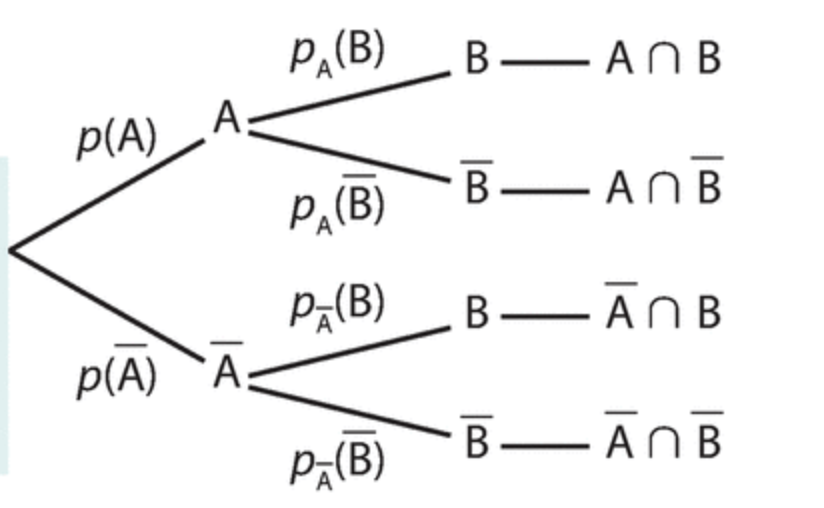
\includegraphics[scale=0.35]{weighted_tree.png}
\end{center}
\property{Parition of universe}
Let $n$ with $n \in \mathbb{N}$ and $n \ge 2$ events of prob $\ne 0$: $A_1,A_2,A_3,...,A_n$ These events format a partition of universe $\Omega$ if:
\begin{itemize}
    \item disjointed two by two $p(A_i \cap A_j) = \O$ if $i \ne j$
    \item $A_1 \cup A_2 \cup ... \cup A_n = \Omega$
\end{itemize}
\property{Weighted tree and partition}
We can build trees with more than 2 branches from the same node as long as all the linked events form a partition of the universe. 
\subsection{Total probability formula}
\property{Total probability formula (peculiar cases)}
Let A such as $p(A) \ne 0$ and $p(\overline{A}) \ne 0$. Probability of B is $$p(B) = p(A \cap B) + p(\overline{A} \cap B) = p(A) \times p_A(B) + p(\overline{A}) \times p_{\overline{A}}(B)$$
\property{Total probability formula (general case)}
Let $A_1, A_2,...,A_n$ and $B_1, B_2, ...,B_m$ two universe partitions. For $i \in [1;m]$ probability of $B_i$ is:
$$p(B_i) = p(A_1 \cap B_i) + p(A_2 \cap B_i) + ... + p(A_n \cap B_i)$$
$$p(B_i) = p(A_1) \times p_{A_1}(B_i) + p(A_2) \times p_{A_2}(B_i) + ... + p(A_n) \times p_{A_n}(B_i)$$
\section{Notion of independence}
\subsection{Independence of two events}
$A$ and $B$ such as $p(A) \ne 0$ and $p(B) \ne 0$
\definition{Independence of two events}
A and B are independent if $p_A(B) = p(B)$
\property{Independence and intersection}
A and B are independent, if and only if, $p(A \cap B) = p(A) \times p(B)$
\property{Independence and contrary events}
If A and B are independent, so $\overline{A}$ and $B$ also are, as well as $\overline{B}$ and $A$ and $\overline{A}$ and $\overline{B}$
\subsection{Succession of independent trials}
N trials can be represented by a weighted tree and by an n entries array.
\end{document}